
Dessine la courbe d'une fonction qui correspond à chaque tableau

\begin{tikzpicture}
\tkzTabInit[lgt=1,espcl=3]{ $x$ / 1,$f $ / 2}
{ $-2$ ,0,3}
\tkzTabVar{+/$1$,-/$-2$,+/$0$ }
\end{tikzpicture}

\begin{tikzpicture}
\tkzTabInit[lgt=1,espcl=2]{ $x$ / 1,$g $ / 2}
{ $-1$ ,1,3,4}
\tkzTabVar{-/$-1$,+/$3$,-/$-1$,+/$2$ }
\end{tikzpicture}

\begin{tikzpicture}
\tkzTabInit[lgt=1,espcl=3]{ $x$ / 1,$h $ / 2}
{ $-1$ ,1,3}
\tkzTabVar{+/$2$,-/$-3$,+/$4$ }
\end{tikzpicture}

\begin{tikzpicture}
\tkzTabInit[lgt=1,espcl=6]{ $x$ / 1,$u $ / 2}
{ $-4$ ,1}
\tkzTabVar{-/$-1$,+/$3$ }
\end{tikzpicture}
